\documentclass[twocolumn]{aastex61}

\newcommand{\vdag}{(v)^\dagger}
\newcommand\aastex{AAS\TeX}
\newcommand\latex{La\TeX}

%% Reintroduced the \received and \accepted commands from AASTeX v5.2
%\received{July 1, 2016}
%\revised{September 27, 2016}
%\accepted{\today}
\submitjournal{ApJL}

\shorttitle{Atmosphere Characterization of WASP-107\lowercase{b}}
\shortauthors{Kreidberg et al.}

\begin{document}

\title{Water, High-Altitude Condensates, and Methane Depletion in the Atmosphere of the Warm Neptune WASP-107\lowercase{b}}

\correspondingauthor{Laura Kreidberg}
\email{laura.kreidberg@cfa.harvard.edu}

\author{Laura Kreidberg}
\affiliation{Harvard Society of Fellows\
78 Mt. Auburn St.\\
Cambridge, MA 02138, USA}
\affiliation{Harvard-Smithsonian Center for Astrophysics\
60 Garden St.\\
Cambridge, MA 02138}
\nocollaboration

\author{Michael Line}
\affiliation{Arizona State University}
\nocollaboration

\author{Caroline Morley}
\altaffiliation{Sagan Fellow}
\affiliation{Harvard-Smithsonian Center for Astrophysics}
\nocollaboration

\author{Kevin Stevenson}
\affiliation{Space Telescope Science Institute}
\nocollaboration


\begin{abstract}
We report a measurement of the near-infrared transmission spectrum of the warm Neptune exoplanet WASP-107b measured with the Hubble Space Telescope Wide Field Camera 3. We detecta water absorption feature (FIXME confidence). The feature is small amplitude, clouds. We combine an interior structure model of the planet with an atmospheric retrieval . We find an upper limit on the atmospheric metallicity of FIXME solar, a cloud deck . 
\end{abstract}

%% Keywords should appear after the \end{abstract} command. 
%% See the online documentation for the full list of available subject
%% keywords and the rules for their use.
\keywords{planets and satellites: individual (WASP-107b), planets and satellites: atmospheres}

%% From the front matter, we move on to the body of the paper.
%% Sections are demarcated by \section and \subsection, respectively.
%% Observe the use of the LaTeX \label
%% command after the \subsection to give a symbolic KEY to the
%% subsection for cross-referencing in a \ref command.
%% You can use LaTeX's \ref and \label commands to keep track of
%% cross-references to sections, equations, tables, and figures.
%% That way, if you change the order of any elements, LaTeX will
%% automatically renumber them.

%% We recommend that authors also use the natbib \citep
%% and \citet commands to identify citations.  The citations are
%% tied to the reference list via symbolic KEYs. The KEY corresponds
%% to the KEY in the \bibitem in the reference list below. 

%Figures and Tables:
% 1.  transit light curves
% 2.  best fit spectrum
% 3.  retrieval results
% 4.  table of transit depths
% 5.  JWST predictions for cloud models 


\section{Introduction} \label{sec:intro}

\section{Observations}
We observed a single transit of WASP-107b with HST's Wide Field Camera 3 (WFC3) instrument on UT 5-6 June 2017.  The transit observation consisted of five HST orbits. At the beginning of each 96-minute orbit, we took an image of the target with the F130N filter (exposure time = 4.2 s). This direct image is used for wavelength calibration. For the remainder of the target visibility period (about 45 minutes), we obtained time series spectra with the G141 grism, which provides low-resolution spectroscopy over the wavelength range $1.1 - 1.7\,\mu$m.  We used the NSAMP=6, SPARS\_25 readout mode (exposure time = 112 s) to optimize the efficiency of the observations, as determined by the \texttt{PandExo\_HST} planning tool\footnote{https://github.com/spacetelescope/PandExo\_HST}.  As is standard for WFC3 observations of bright targets, we used the spatial scanning observing mode, which slews the telescope in the spatial direction over the course of an exposure. The scan rate was 0.12 arcseconds/sec.


\section{Data Reduction}
We reduced the data with the custom pipeline described in \cite{kreidberg14a}, which we summarize briefly here. For each exposure, we extracted the spectrum from each up-the-ramp sample (or ``stripe") separately using the optimal extraction algorithm of \cite{horne86}. The stripe spectra were then summed to create the final spectrum. For each stripe, the extraction box was 80 pixels high and centered on the stripe's midpoint in the spatial direction. To correct the change in dispersion solution over the length of the spatial scan, we interpolated each row to the wavelength scale of the row corresponding to the spectral trace. We then corrected for slight drift in the spectral direction ($<0.1$ pixels) by interpolating each spectrum to the wavelength scale of the first exposure.  To subtract the background, we took the median of sky pixels that were uncontaminated by the target spectrum (rows $5-250$, columns $5-15$). The typical background counts were low: 40 photoelectrons/pixel, in comparison to $3\times10^4$ photoelectrons/pixel in the stellar spectrum.
%dispersion solution: 46 Angstroms/pixel. max drift: 3 angstroms (from diagnostics.txt)

\section{Light Curve Analysis}
The data analysis had two parts: the band-integrated ``white" light curve fit and the spectroscopic light curve fits.

\subsection{White Light Curve}
To create the raw white light curve, we summed each spectrum over the 181 pixels in the spectral trace.  The white light curve has systematic trends that are typical for WFC3 observations \citep{zhou17}: the flux increases increases asymptotically over each orbit (the ``ramp" effect) and there is a visit-long linear trend. The largest ramp occurs in the initial orbit (orbit zero), so we only fit data from orbits one through four in our analysis, following common practice.  We fit the light curve with the analytic model of the form $F_\mathrm{white}(t) = S_\mathrm{white}(t)\times T_\mathrm{white}(t)$, where $S_\mathrm{white}$ is a systematics model and $T_\mathrm{white}$ is a transit model. We used the same systematics model as \cite{kreidberg15b}, Equation 1.  To model the transit, we used the \texttt{batman} package \citep{kreidberg15a}.  The transit model parameters are the orbital period $p$, time of inferior conjunction $t_0$, transit depth $r_p/r_s$, ratio of semi-major axis to stellar radius $a/r_s$, orbital inclination $i$, and the quadratic stellar limb darkening parameters $u_1$ and $u_2$.

\begin{figure*}
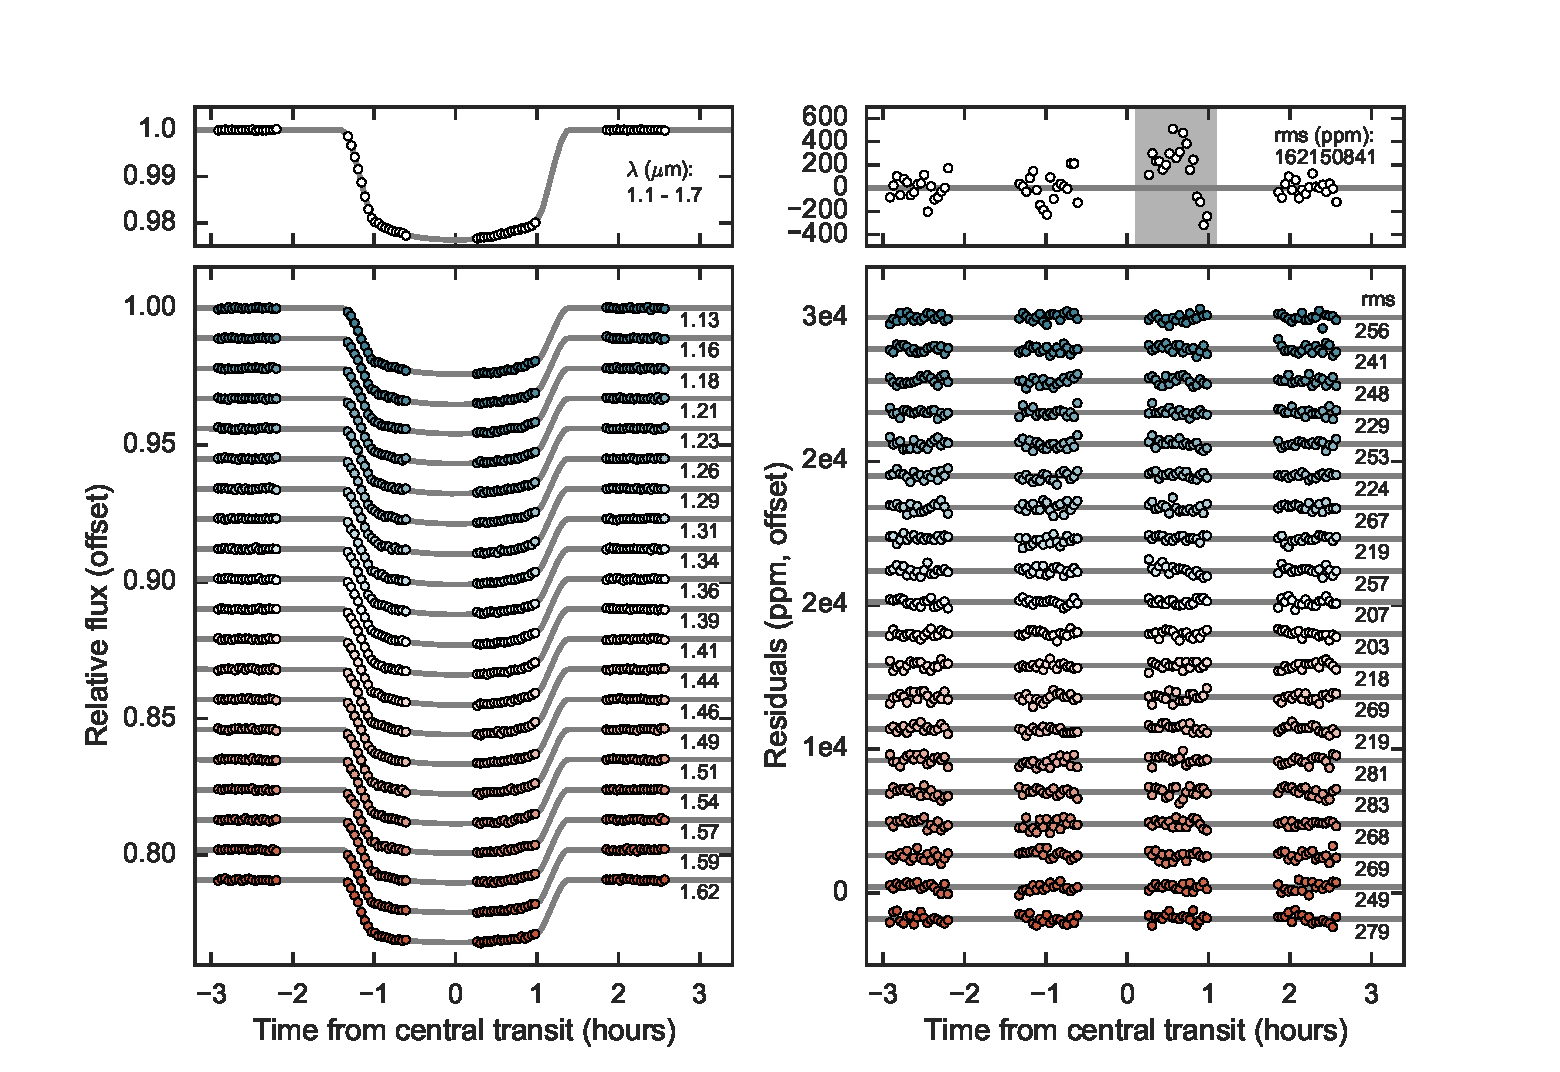
\includegraphics[width = \textwidth]{Figures/lc.pdf}
\caption{FIXME}
\label{fig:lc}
\end{figure*}

\subsubsection{Star Spot Crossing}
In our initial analysis, we noticed a bump in the light curve during orbit three that was not fit well with our model. We attribute this feature to a star spot crossing event, as WASP-107 is an active star and spot crossings have been observed before \citep{dai17, mocnik17}. In our subsequent analysis, we gave the data in orbit three no weight in the fit. The amplitude of the spot crossing feature is 300 ppm, as illustrated in Figure\,\ref{fig:lc}.

\subsubsection{Final Fit}
In our final fit, we fixed the transit parameters $a/r_s$, $i$, $p$ on the precise estimates from the Kepler light curve \citep{dai17}.  These values are consistent with our best fit when we allowed them to vary freely. We also fixed the limb darkening parameters on predictions from a PHOENIX model for a star with effective temperature 4300 K, calculated with the \texttt{limb-darkening} package from \cite{espinoza15}.  The remaining free parameters were $t_0$, $r_p/r_s$, and the systematics parameters for the visit-long and orbit-long trends.
%The model values are consistent with what we obtain from fitting for the limb darkening coefficients as free parameters. 

For the best fit white light curve, the root-mean-square (rms) residuals were 93 ppm (excluding the star spot crossing), which is somewhat larger than the expected shot noise of 50 ppm. We attribute the excess noise to loss of flux off the edge of the detector, which can occur if there is variation in the position or length of the spatial scan. There is no evidence for correlated noise in the residuals, so to account for the excess noise we simply increased the per-point uncertainties by a factor of 1.7 to achieve a reduced $\chi^2$ value of unity.  We then used the Markov chain Monte Carlo (MCMC) algorithm to estimate parameter uncertainties \citep{foremanmackey13}.  The chain had 50 walkers which each ran for $10^4$ steps with the first 10\% discarded as burn-in. We tested for convergence by dividing the chain in two halves and confirming that they gave consistent results. The transit time was $t_0 = 2457910.45407\pm6\mathrm{e}{-5}$ BJD$_\mathrm{TDB}$ and the planet/star radius was $r_p/r_s = 0.14399\pm0.00017$. 

\subsection{Spectroscopic Light Curve Fits}
We binned the spectrum into 20 spectrophotometric channels from 1.12 to 1.65 $\mu$m, shown in Figure\,\ref{fig:lc}. We fit the light curves with the \texttt{divide-white} technique, which assumes that the light curve systematics have the same morphology at all wavelengths \citep{stevenson14c, kreidberg14a}. For this method, the transit model $T_\lambda(t)$ is multiplied by the systematics vector from the white light curve fit ($F_\mathrm{white}/T_\mathrm{white}$), and rescaled by a factor $C_\lambda + V_\lambda t$.  One advantage of this approach is that it removes the star spot crossing feature, enabling us to use orbit three with no additional correction. The amplitude of the feature has no detectable wavelength dependence at the level of precision of our data.  As for the white light curve, we fixed some of the transit parameters on the estimates from \cite{dai17} and fixed the limb darkening on the PHOENIX model. The final spectroscopic light curve fits had just three free parameters: $C_\lambda$, $V_\lambda$, and $r_p/r_s$.  

The best fit light curves have a median reduced $\chi^2$ value of 1.16.  To ensure that we did not underestimate the uncertainty on the transit depths, we rescaled the photometric uncertainties for all spectroscopic channels such that the $\chi^2$ values are unity. We performed an MCMC fit to the light curves with \texttt{emcee}.  For each light curve we ran a fit with 50 walkers and 1000 steps per walker, and tested for convergence as we did for the white light curve. The median transit depths and $1\,\sigma$ uncertainties are given in Table\,\ref{tab:transit_depths}. 

We explored several alternative choices for the spectroscopic light curve fits, but found that none of them made a significant difference in the transmission spectrum. For example, we fit the spectroscopic light curves with the same analytic model we used for the white light curve and obtained nearly identical relative transit depths (differing by just $0.3\sigma$ on average), except with a small constant offset due to the uncorrected star-spot crossing feature. This offset does not affect our final analysis because the planet's one-bar radius is a free parameter in the atmospheric retrieval (see \S\,\ref{sec:retrieval}). We also fit for a linear limb darkening parameter rather than fixing the limb darkening on the PHOENIX model values. We found that the fitted limb darkening coefficients are consistent with the model predictions, so we opted to fix the coefficients in our final analysis because it improves the precision on the transit depths by about 10\%. We also checked that the uncertainty in the stellar parameters does not significantly affect the PHOENIX model predictions at the level of precision of our data. 

\subsubsection{Transit Depths Redder than 1.62 $\mu$m}
The red edge of the transmission spectrum is of interest for our analysis because methane is expected to be the dominant absorber over water at wavelengths greater than $1.6\,\mu$m. Unfortunately, we find that the our reddest spectroscopic light curves ($>1.62\mu$m) are too poor in quality to robustly measure the transit depth. The residuals exhibit correlated noise and the fits have reduced $\chi^2_\nu>2$. The transit depths are also sensitive to which method we use to fit for instrument systematics.  We therefore opt not to report transit depths redder than the 1.62 $\mu$m channel.

\subsubsection{Independent Analysis}
We also performed an independent data reduction and fit using K. Stevenson's pipeline.

\begin{figure*}
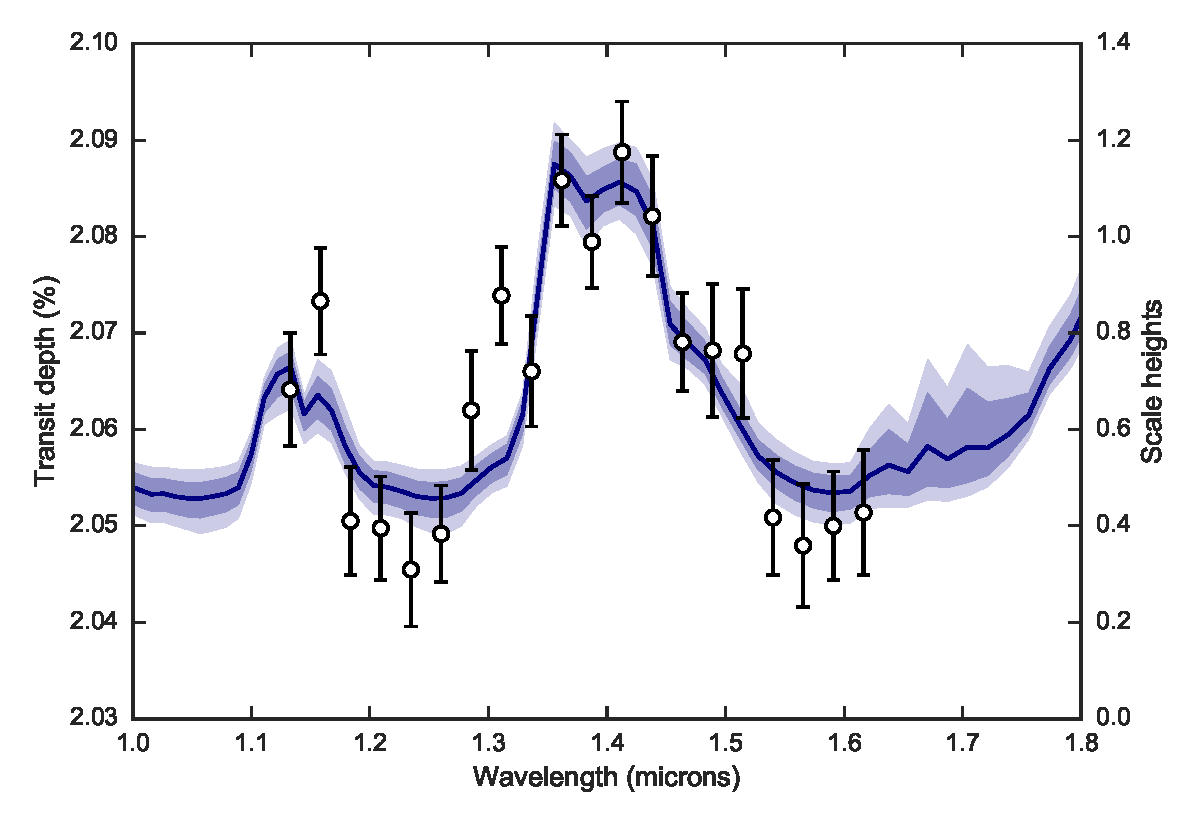
\includegraphics[width = \textwidth]{Figures/spectrum.pdf}
\caption{FIXME}
\label{fig:spectrum}
\end{figure*}

\begin{deluxetable}{c c c}
\tablecaption{WASP-107b transmission spectrum \label{tab:transit_depths}}
\tablehead{\colhead{Wavelength ($\mu$m)}  & \colhead{Transit depth} & \colhead{Uncertainty}}
\startdata
1.133 & 0.020641 & 5.9e-05 \\
1.158 & 0.020733 & 5.5e-05 \\
1.184 & 0.020505 & 5.6e-05 \\
1.209 & 0.020498 & 5.4e-05 \\
1.235 & 0.020455 & 5.9e-05 \\
1.260 & 0.020492 & 5.0e-05 \\
1.285 & 0.020620 & 6.2e-05 \\
1.311 & 0.020739 & 5.0e-05 \\
1.336 & 0.020660 & 5.7e-05 \\
1.362 & 0.020858 & 4.8e-05 \\
1.387 & 0.020794 & 4.8e-05 \\
1.413 & 0.020888 & 5.2e-05 \\
1.438 & 0.020821 & 6.2e-05 \\
1.464 & 0.020691 & 5.1e-05 \\
1.489 & 0.020682 & 6.9e-05 \\
1.515 & 0.020679 & 6.7e-05 \\
1.540 & 0.020509 & 6.0e-05 \\
1.565 & 0.020480 & 6.4e-05 \\
1.591 & 0.020500 & 5.6e-05 \\
1.616 & 0.020514 & 6.5e-05 \\
\enddata
\end{deluxetable}

\section{Composition of the Atmosphere}
In this section we discuss constraints on the composition of WASP-107b's atmosphere based on interior structure modeling and atmospheric retrieval of the measured transmission spectrum.

\subsection{Atmospheric Metallicity from Interior Structure Modeling}
Given WASP-107b's unusually low density, we sought to estimate the range of atmospheric metallicities that are consistent with the observed mass and radius.  We estimated the bulk metallicity of WASP-107b using the structure evolution modeling of \cite{thorngren16}.  These models assume a thermally inert heavy-element core with a convective envelope of additively mixed H/He \citep{saumon95} and heavy-element impurities.  The heavy elements were a 50-50 rock-ice mix from ANEOS \citep{thompson90}.  We evolved the planets in time using the atmospheric models of \cite{fortney07}.  The results are sensitive to assumptions about the stellar age, which is uncertain \citep[either $0.6\pm0.2$ to $8.3\pm4.3$ Gyr depending on model assumptions;][]{mocnik17}. We therefore ran two models, with uniform age priors of either $0.2-1.0$ or $1.0-13.8$ Gyr.  We used the published mass and radius estimates \citep[$0.12\pm0.01\,M_\mathrm{J}$, $0.94\pm0.02$;][]{anderson17}.  A more precise mass estimate is in preparation (B. Benneke, priv.\,comm.); however, we find that our results are not signficantly affected when we vary the assumed mass by $\pm3\,\sigma$ from the published value because the dominant uncertainties are the stellar age and core mass.

Based on these assumptions, we fit for envelope metallicity and core mass using an MCMC with uniform priors on both parameters.  The MCMC burned in for $10^3$ steps and then collected $4\times10^6$ samples, which we thinned to $10^5$.  The resulting envelope metal mass fractions were converted to metallicities by assuming the mean molecular weight of the metals was about 18 (the value for water), using the approach of \cite{fortney13}. Figure\,\ref{fig:metal_prior} shows the results.  We find that the inferred atmospheric metallicity and core mass are inversely proportional, as expected (the more massive the core, the lighter the envelope must be to maintain the observed radius). Larger core masses and envelope metallicities are allowed for the younger stellar age (when planets age, they cool and contract).  For the younger (older) stellar age, we find an upper limit on the core mass of FIXME and an upper limit on atmospheric metallicity of FIXME.

\begin{figure}
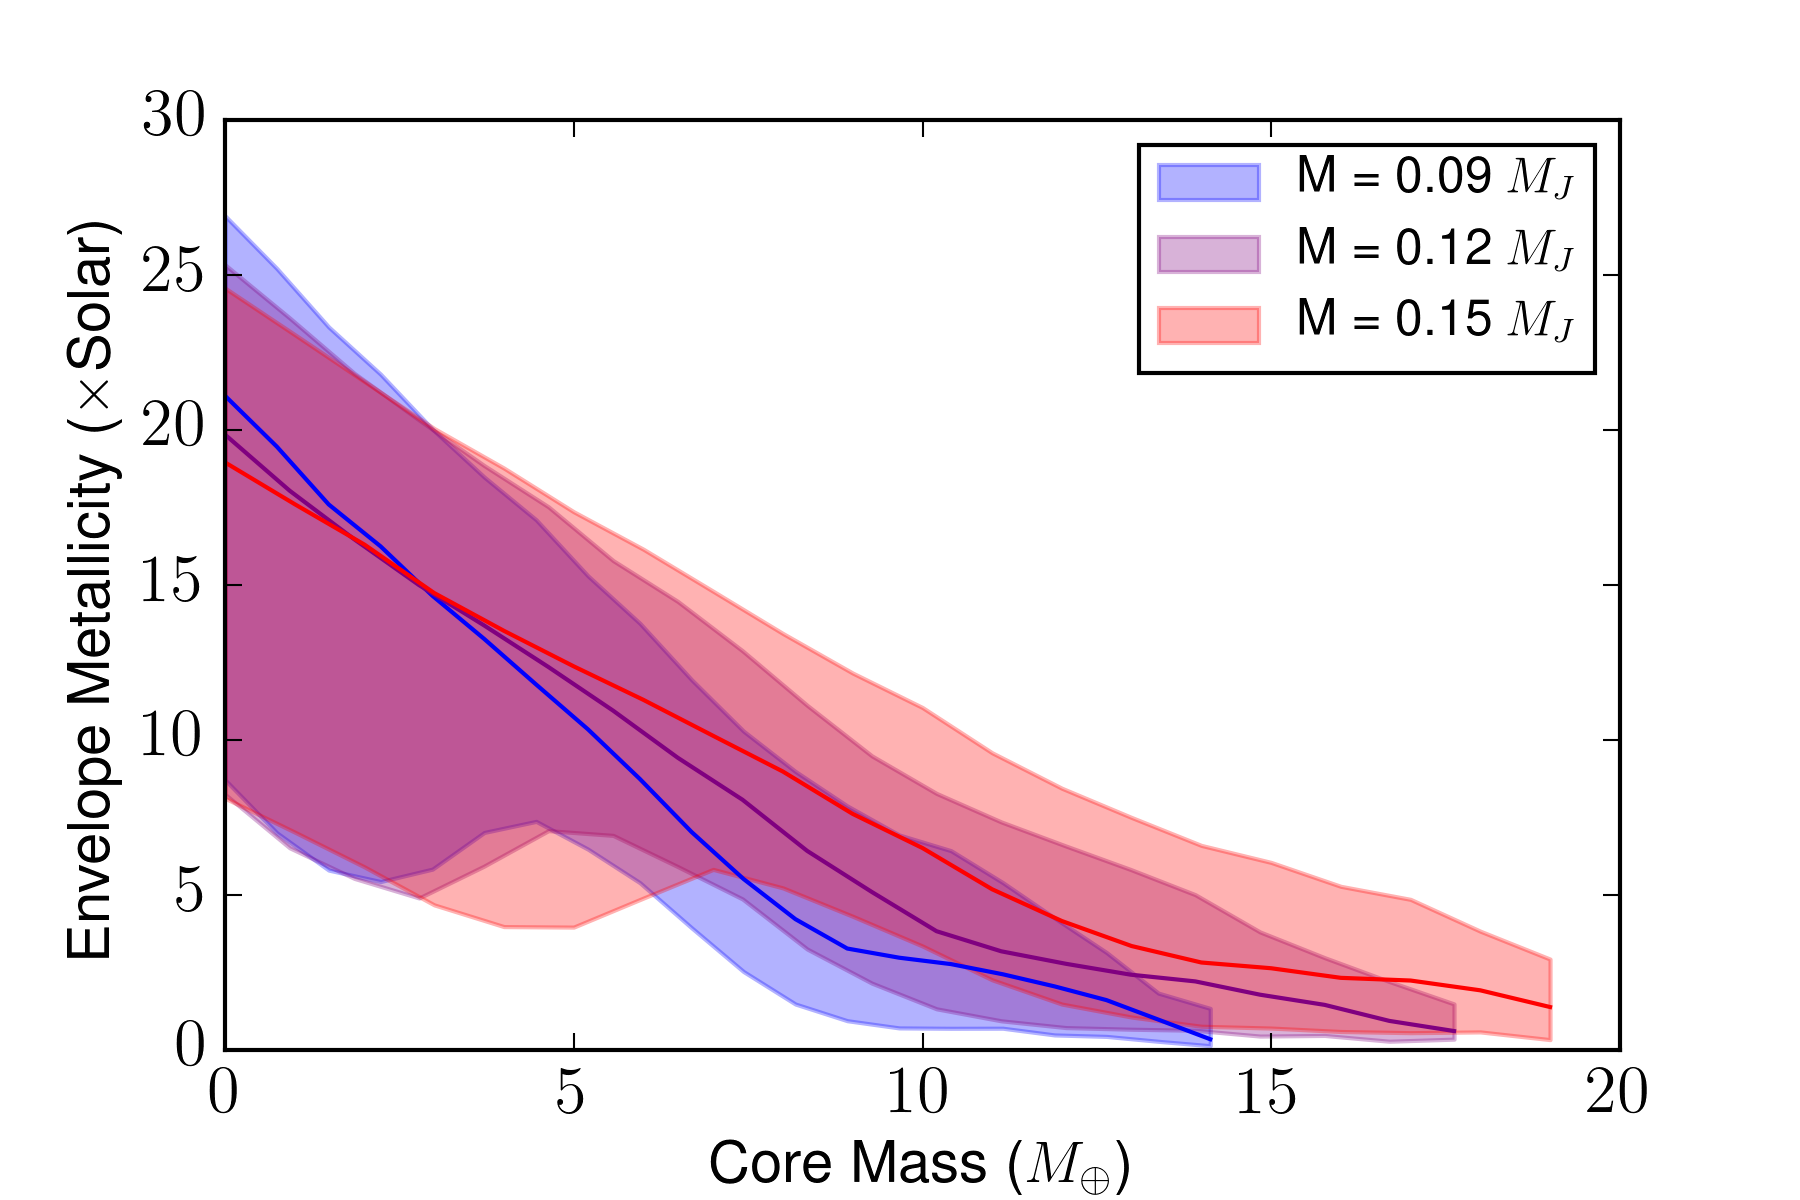
\includegraphics[width = 0.5\textwidth]{Figures/metalByMass.png}
\caption{FIXME}
\label{fig:metal_prior}
\end{figure}

\subsection{Retrieval}
\label{sec:retrieval}
We used the CHIMERA chemically-consistent retrieval tool described in \cite{kreidberg15b} to determine the planet's basic atmospheric properties from the transmission spectrum.   Briefly, CHIMERA solves the transmission geometry problem using the equations in \cite{brown01, tinetti12}.  We parameterize atmospheric composition with metallicity and carbon-to-oxygen ratio (C/O) under the assumption of thermochemical equilibrium using the NASA CEA routine \citep{gordon96} to compute the molecular abundances for H$_2$, He, H$_2$O, CH$_4$, CO, CO$_2$, NH$_3$, H$_2$S, Na, K, HCN, C$_2$H$_2$, TiO, VO, and FeH.    We recently upgraded the transmission model to use correlated-K opacities \citep{lacis91, molliere15, amundsen16} for the aforementioned gases generated from the pre-tabulated line-by-line cross section database described in \cite{freedman14}. The transmission forward model is coupled with the powerful PyMultiNest tool \citep{buchner16} to solve the parameter estimation and model selection problems.  

The nominal model set-up requires a temperature-pressure profile (parameterized via the \citealt{guillot10} relations), the atmospheric metallicity and carbon-to-oxygen ratio for molecular composition determination, disquilibrium properties crudely parameterized with nitrogen species and carbon species quench pressures \citep{morley17}, and aerosol properties.  We experiment with three atmospheric scenarios within this setup: scenarios with and without methane, and with/without patchy cloud cover (as described and implemented in \citealt{line16}.  In all three scenarios we fix the T-P profile ``shape" but scale the irradiation temperature, to allow for the unknown albedo and heat transport efficiency.  T-P profile shape information is not readily retrievable, nor does it strongly influence information derived from WFC3 transmission spectra \citep[e.g.][]{kreidberg15b}.  Aerosols are parameterized with a ``gray cloud top pressure" with the option for cloud patchiness. %We do not consider ``sloped hazes" at this time as they are unlikely to influence the results.
%We also switch off the quench pressure parameters as they are unlikely to strongly influence the equilibrium abundance profiles of the spectrally prominent, nearly constant-with-altitude abundance, species like CH$_4$, H$_2$O, and NH$_3$ over this temperature range \citep[e.g.][]{line11, moses13}.  

\section{Discussion} \label{sec:discuss}


We note that some directly imaged self-luminous planets in this temperature regime are also unexpectedly depleted in methane when compared to similar temperature brown dwarfs \citep{skemer14}.   The leading hypothesis of this depletion \citep{zahnle14} is due to the CH4-CO quench point occurring in the CO stability field due to the low gravity of self-luminous planets when compared to brown dwarfs.  In order this mechanism to work for neptune massed planet, the internal temperature would have to be near ~500K to get the deep temperatures high enough to thermochemically deplete methane at the quench point. Given the age of the star, it is unlikely that such high internal temperatures are still due to heat of formation. It is possible that tidal heating could increase the internal temperature (Agundez et al. 2014; Morley et al. 2017) but that would require a negligible eccentricity, of which is currently uncertain for WASP107b.


\subsection{Methane}

\subsection{Comparative planetology with HAT-P-11b, HAT-P-26b}

\subsection{Constraints on Condensate Properties}
The amplitude of WASP-107b's spectral features is about half that expected for an atmosphere free of condensates. In our retrieval analysis, we explored two simple parameterizations to model condensates: a gray opacity source and a sloped haze.  The retrieved cloud-top pressure is FIXME at $1\,\sigma$ confidence.

We also considered physically motivated, self-consistent cloud and haze models based on .  To model WASP-107b's spectrum with self-consistent aerosols, we use the methods described in \citep{fortney08, morley15}. We include models from solar to $50\times$ solar metallicity and solar C/O ratio. We model clouds that form in cool atmospheres (Na$_2$S, KCl, ZnS, see \citealt{morley12}), varying the cloud sedimentation efficiency from 0.1 to 3. None of the cloudy models are sufficiently low amplitude to match the observed muted signal. We also model an ad hoc photochemical 'soot' layer near the top of the atmosphere, scaling results from previous photochemical models for GJ 436b \citep{line11, morley17}. With a sufficiently thick photochemical haze with particle sizes around $0.03-0.1$ microns, the amplitude of the model water feature matches that of the observations. 





\section{Future Plans}
WASP-107b is slated to be observed with numerous facilities. Transits were recently observed with the WFC3/G102 grism and Spitzer 3.6 and 4.5 $\mu$m channels. Spitzer eclipses are planned (Program FIXME; PI L. Kreidberg). In addition, WASP-107b is included in the \emph{JWST} Guaranteed Time Observations.

Combine data from Spitzer/HST
JWST GTO


\acknowledgments
Fei Dai
Jessica Spake

L.R.K. acknowledges support from the Harvard Society of Fellows and the Harvard Astronomy Department Institute for Theory and Computation.

\vspace{5mm}
\facilities{HST(WFC3)}

%% Similar to \facility{}, there is the optional \software command to allow 
%% authors a place to specify which programs were used during the creation of 
%% the manusscript. Authors should list each code and include either a
%% citation or url to the code inside ()s when available.

%\software{astropy \citep{2013A&A...558A..33A},  
%          Cloudy \citep{2013RMxAA..49..137F}, 
%          SExtractor \citep{1996A&AS..117..393B}
%          }

%% Appendix material should be preceded with a single \appendix command.
%% There should be a \section command for each appendix. Mark appendix
%% subsections with the same markup you use in the main body of the paper.

%% Each Appendix (indicated with \section) will be lettered A, B, C, etc.
%% The equation counter will reset when it encounters the \appendix
%% command and will number appendix equations (A1), (A2), etc. The
%% Figure and Table counter will not reset.

%\appendix


%% The reference list follows the main body and any appendices.
%% Use LaTeX's thebibliography environment to mark up your reference list.
%% Note \begin{thebibliography} is followed by an empty set of
%% curly braces.  If you forget this, LaTeX will generate the error
%% "Perhaps a missing \item?".
%%
%% thebibliography produces citations in the text using \bibitem-\cite
%% cross-referencing. Each reference is preceded by a
%% \bibitem command that defines in curly braces the KEY that corresponds
%% to the KEY in the \cite commands (see the first section above).
%% Make sure that you provide a unique KEY for every \bibitem or else the
%% paper will not LaTeX. The square brackets should contain
%% the citation text that LaTeX will insert in
%% place of the \cite commands.

%% We have used macros to produce journal name abbreviations.
%% \aastex provides a number of these for the more frequently-cited journals.
%% See the Author Guide for a list of them.

%% Note that the style of the \bibitem labels (in []) is slightly
%% different from previous examples.  The natbib system solves a host
%% of citation expression problems, but it is necessary to clearly
%% delimit the year from the author name used in the citation.
%% See the natbib documentation for more details and options.

\bibliographystyle{aasjournal}
\bibliography{ms.bib}

%% This command is needed to show the entire author+affilation list when
%% the collaboration and author truncation commands are used.  It has to
%% go at the end of the manuscript.
%\allauthors

%% Include this line if you are using the \added, \replaced, \deleted
%% commands to see a summary list of all changes at the end of the article.
%\listofchanges

\end{document}

% End of file `sample61.tex'.
